\documentclass[main.tex]{subfiles}

\begin{document}
\chapter{Central Results}
\lhead{Central Results}

\section{English LUKE Reproduction}%
\label{sec:English LUKE Reproduction}
\begin{table}[H]
	\begin{center}
		\begin{tabular}{l c c c c c}
			Model & Micro avg. & LOC & PER & ORG & MISC \\
			\hline
			LUKE large & $94.00 \pm  0.2$ & $94.99 \pm  0.09$ & $97.19 \pm  0.1$ & $93.63 \pm  0.3$ & $85.29 \pm  1$ \\
			LUKE base & $93.42 \pm  0.2$ & $94.67 \pm  0.2$ & $96.89 \pm  0.2$ & $92.41 \pm  0.2$ & $84.94 \pm  0.7$ \\
			 &  &  &  &  &  \\
			Support & 5616 & 1666 & 1602 & 1647 & 701 \\
		\end{tabular}
	\end{center}
	\caption{Mean F1\pro\ scores and standard deviation over five repetitions of fine-tuning and evaluating LUKE on CoNLL2003 for each model size.}
%    TODO: If not already, it should be stated somewhere that all multiclass F1 refer to micro average
	\label{tab:lukeF1s}
\end{table}

\section{Pretraining of daLUKE}%
\label{sec:Pretraining of daLUKE}
\begin{enumerate}
    \item Resultater for maskerede opgaver
    \item Alle træningskurverne for hovedeksperimentet
\end{enumerate}

\begin{table}[H]
    \centering
    \begin{tabular}{l|rrrrrr}
        Top $k$ accuracy [\pro] & $k=1$  & $k=3$ & $k=5$ & $k=10$ & $k=25$ & $k=50$\\\hline
        Masked words            & 24.82       & 31.54      & 34.96      & 40.27       & 48.15       & 54.02      \\
        Masked entities         & 56.17       & 68.58      & 73.58      & 79.78       & 86.36       & 90.27
    \end{tabular}
    \caption{
        The main pretrained model performance in the last of 150 epochs.
        The measures are frequency of correct prediction on the two mask prediction tasks, when considering a prediction to be correct if the true token is one $K$ most likely labels according to the model softmax output.
    }
    \label{tab:mainpre}
\end{table}\noindent

\begin{figure}[H]
    \centering
    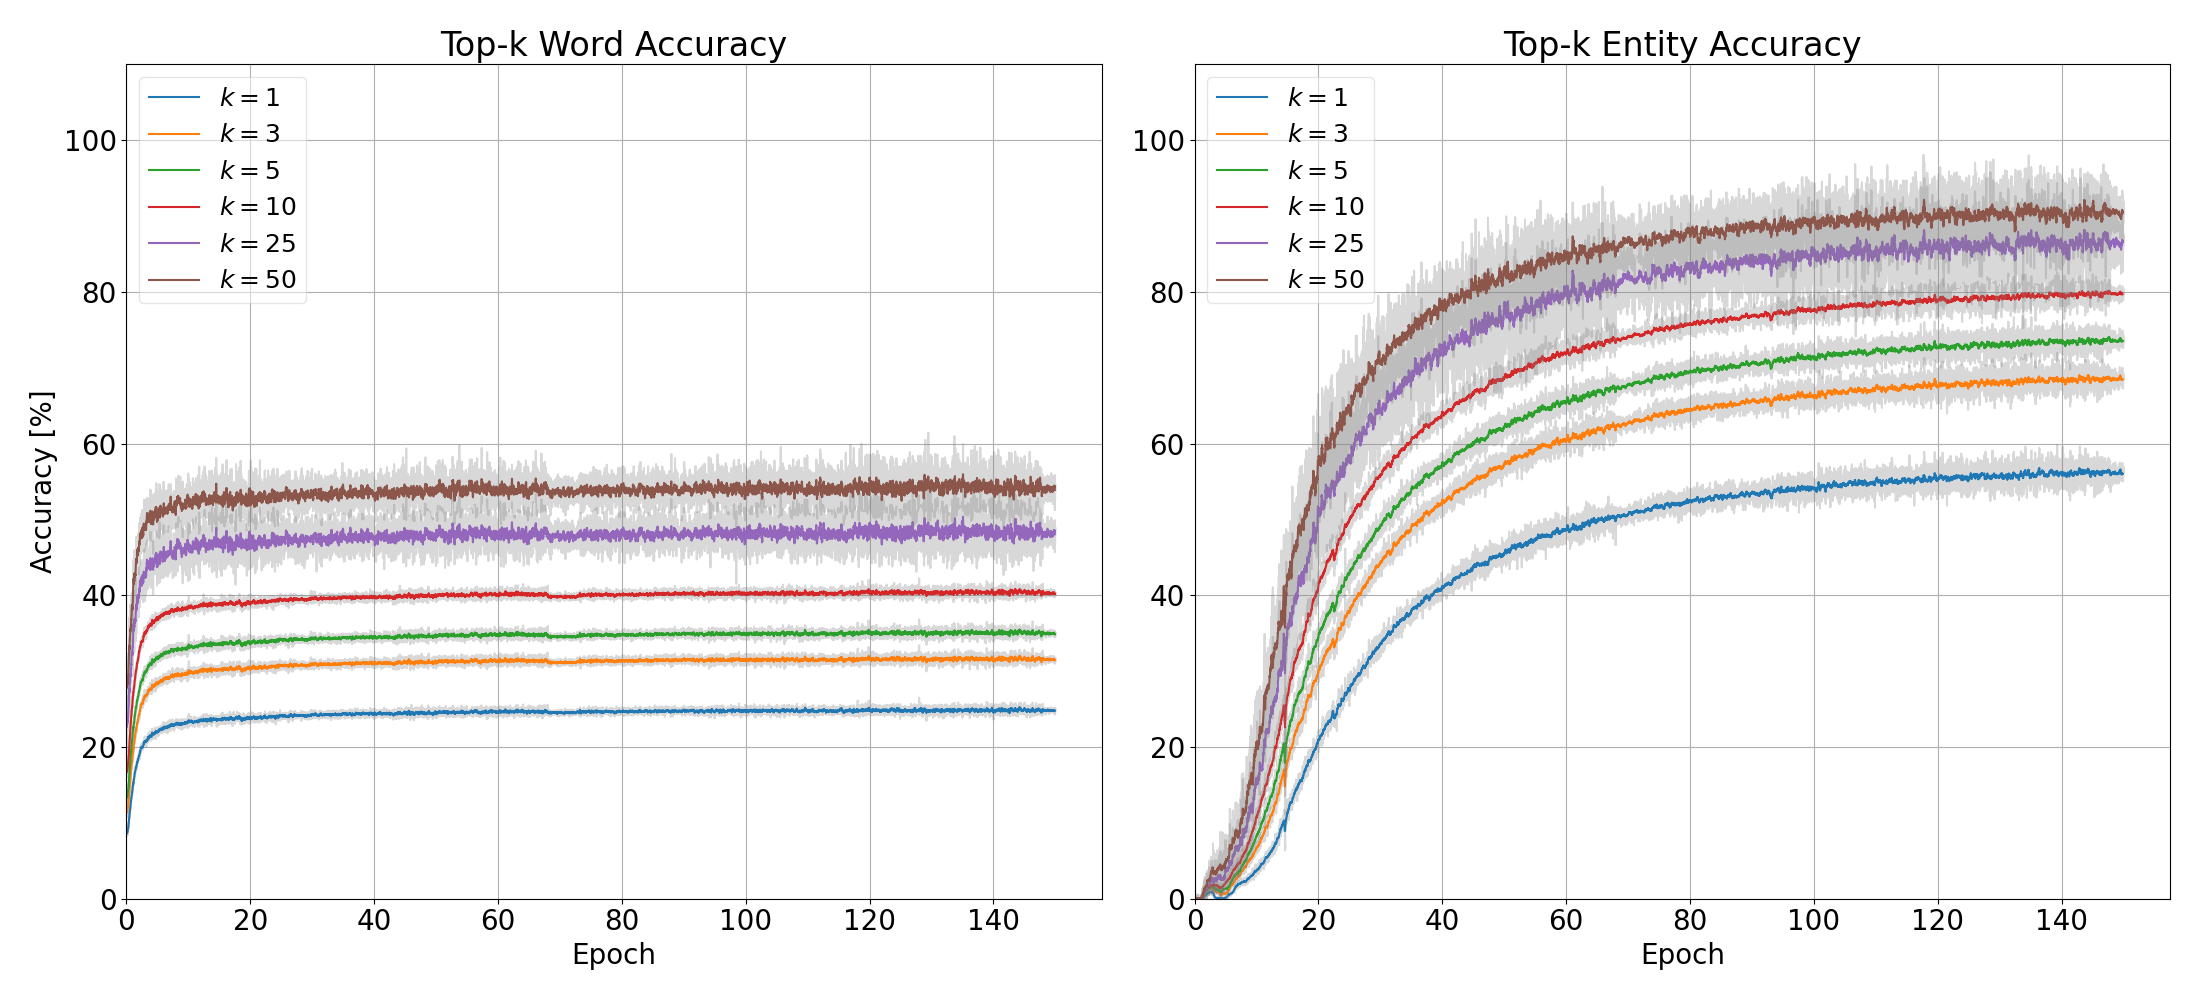
\includegraphics[width=0.8\textwidth]{pretrain-acc}
    \caption{Masked sub-words and masked entity accuracy throughout pretraining.}
    \label{fig:pretrain-acc}
\end{figure}\noindent

\section{Danish Named Entity Recognition}%
\label{sec:nerres}
\begin{table}
        \begin{center}                     
                \begin{tabular}{l l r r r r r r}                                                                                                                                                                                        
                        Model & Train. data & Micro avg. & ⁒MISC & LOC & PER & ORG & MISC \\                                                                                                                                          
                        \hline                                                                                                                                                                                                          
                        DaNLP da-BERT & DaNE & - & 84.04 & 83.90 & 92.82 & 72.98 & - \\                                                                                                                                                 
                        NERDA m-BERT & DaNE & 79.22 & 81.71 & 83.50 & 92.61 & 66.90 & 70.34 \\                                                                                                                                          
                        NERDA Ælæctra & DaNE & 70.58 & 74.54 & 77.32 & 86.93 & 56.18 & 56.39 \\                     
                        DaCy & DaNE & 84.91 & 86.89 & 85.29 & 94.15 & 79.04 & 78.05 \\                              
                        DaNLP spaCy & DaNE & 73.75 & 75.73 & 75.96 & 87.87 & 59.57 & 66.06 \\                       
                        DaNLP Flair & DaNE & - & 81.78 & 84.82 & 93.15 & 62.95 & - \\                               
                        Polyglot & Wikipedia & - & 64.18 & 64.95 & 78.74 & 39.30 & - \\                             
                        DKIE Stanford CRF & ITU CDT & - & 56.52 & 59.49 & 70.40 & 28.29 & - \\                      
                         &  &  &  &  &  &  &  \\          
                        Support &  & 558 & 437 & 96 & 180 & 161 & 121 \\                                            
                \end{tabular}                             
        \end{center}                                      
        \caption{F1\pro-scores of Danish NER models of the DaNE data-set consisting of 565 sentences.}              
        \label{tab:DaNE}                                  
\end{table}                                               
\begin{table}                                             
        \begin{center}                                    
                \begin{tabular}{l l r r r r r r}          
                        Model & Train. data & Micro avg. & ⁒MISC & LOC & PER & ORG & MISC \\                      
                        \hline                            
                        DaNLP da-BERT & DaNE & - & 79.23 & 78.64 & 93.45 & 56.88 & - \\                             
                        NERDA m-BERT & DaNE & 66.37 & 76.60 & 76.33 & 92.08 & 52.53 & 12.41 \\                      
                        NERDA Ælæctra & DaNE & 66.28 & 76.09 & 74.87 & 90.32 & 53.00 & 13.24 \\                     
                        DaCy & DaNE & 68.45 & 79.02 & 79.02 & 92.53 & 58.04 & 15.48 \\                              
                        DaNLP spaCy & DaNE & 64.11 & 72.70 & 72.73 & 88.33 & 46.51 & 12.31 \\                       
                        DaNLP Flair & DaNE & - & 76.16 & 80.21 & 94.35 & 36.96 & - \\                               
                        Polyglot & Wikipedia & - & 64.10 & 69.74 & 78.38 & 24.69 & - \\                             
                        DKIE Stanford CRF & ITU CDT & - & 59.89 & 58.16 & 73.63 & 26.09 & - \\                      
                         &  &  &  &  &  &  &  \\          
                        Support &  & 390 & 360 & 97 & 169 & 94 & 30 \\                                              
                \end{tabular}                             
        \end{center}                                      
        \caption{F1\pro-scores of Danish NER models of the Plank data-set consisting of 565 sentences.}             
        \label{tab:Plank}                                 
\end{table}                                               

\begin{table}                                             
        \begin{center}                                    
                \begin{tabular}{l l r r r r}              
                        Model & Train. data & Micro avg. & LOC & PER & ORG \\                                       
                        \hline                            
                        DaNLP da-BERT & DaNE & 65.66 & 72.08 & 74.49 & 40.05 \\                                     
                        NERDA m-BERT & DaNE & 63.40 & 70.72 & 76.87 & 48.35 \\                                      
                        NERDA Ælæctra & DaNE & 48.65 & 56.63 & 69.89 & 24.02 \\                                     
                        DaCy & DaNE & 64.55 & 74.11 & 77.18 & 49.78 \\                                              
                        DaNLP spaCy & DaNE & 59.55 & 68.68 & 71.63 & 38.76 \\                                       
                        DaNLP Flair & DaNE & 65.04 & 70.08 & 74.36 & 43.67 \\                                       
                        Polyglot & Wikipedia & 61.99 & 72.45 & 69.15 & 35.33 \\                                     
                        DKIE Stanford CRF & ITU CDT & 46.59 & 56.15 & 54.51 & 14.76 \\                              
                         &  &  &  &  &  \\                
                        Support &  & 13698 & 5242 & 4378 & 4078 \\                                                  
                \end{tabular}                             
        \end{center}                                      
        \caption{F1\pro-scores of Danish NER models of the WikiANN data-set consisting of 10000 sentences.}         
        \label{tab:WikiANN}                               
\end{table}                                               

\end{document}
